\section{Demonstrating the strength of the suggested approach -- a case study}
\label{sec:casestudy}

The case study presented in this section, which was first published in
\cite{Wandeler&04} using other analysis techniques, is inspired by a
system architecture definition study for a new distributed in-car radio
navigation system. Such a system typically executes a number of concurrent
software applications that share a common
hardware platform. Each application might have hard individual performance
requirements that need to be met. During the system definition phase, several
candidate platform architectures are proposed by the engineers and the system
architect needs to evaluate all of them and decide which one to implement. The
system architect makes these decisions by building and analyzing models that
support the design choices. From our own experience, the success of this
activity is very much dependent on the amount of time needed to perform the
work. Time-to-market targets are hard, especially so in the embedded systems
domain and modelling and analysis techniques that do not meet this requirement
are simply not used in practice, even despite their potential \textsc{[Dana]}.

\begin{figure}[htb]
\begin{center}
\vspace{-0.8cm}
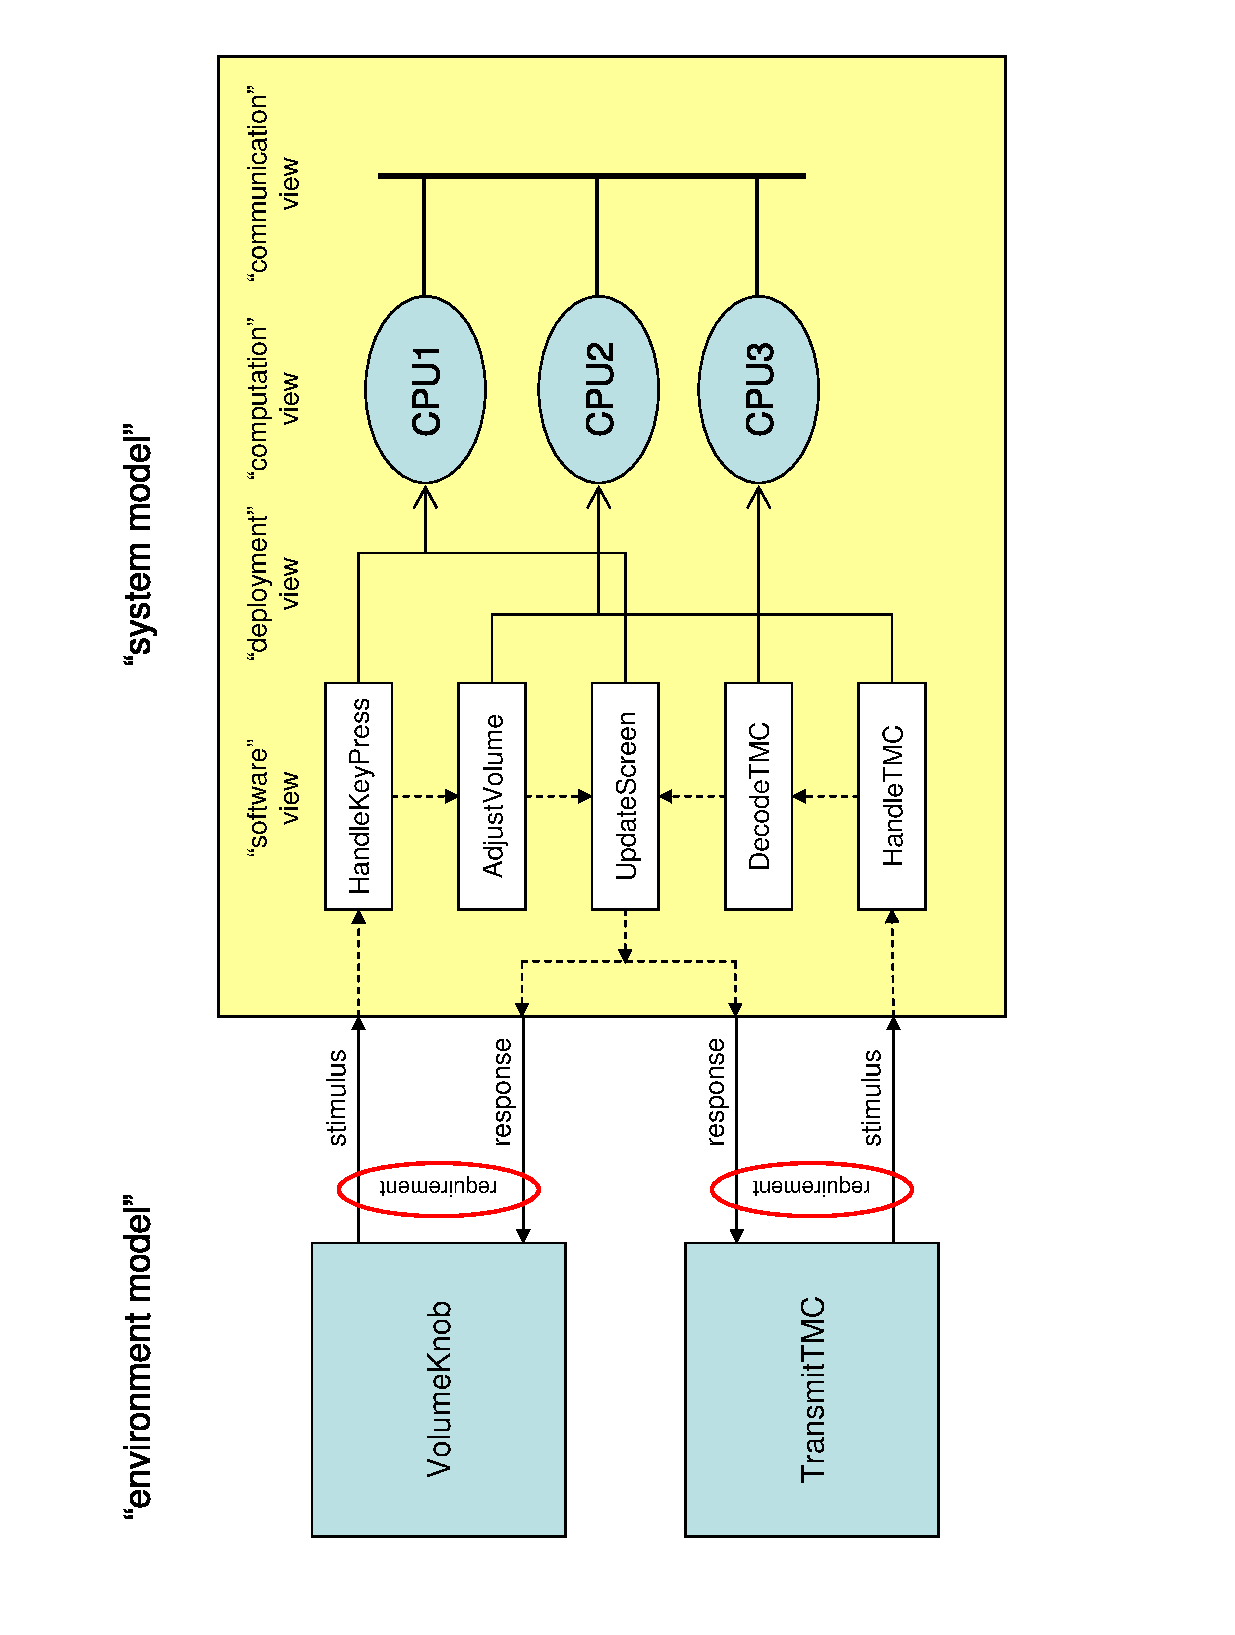
\includegraphics[width=0.6\columnwidth,angle=-90]{casestudy.eps}
\vspace{-1.5cm}
\caption{An overview of the case study}
\label{fig:casestudy}
\end{center}
\end{figure}

The in-car radio navigation system contains many applications, we will
consider just two of them here because of space limitations; the full
model is available in \textsc{[TechRep]}. An informal overview of the
case study is presented in Figure~\ref{fig:casestudy}. An embedded system,
as its name suggests, needs to be described in combination with its
environment. In our model, we partition the \textit{world} into an
\textit{environment model} and a \textit{system model}.

In our case study, there are two tasks that represent the environment.
They independently inject stimuli into the system and observe its response.
The rate at which these events are generated can for example be described by
the triple $(p,j,d)$ where $p$ represents the period, $j$ the jitter and
$d$ the minimum time between two consequtive events. Typically system-level
temporal and timing requirements can be specified at this interface. Informal
examples of these requirements are respectively: \textit{``The order of the
input stimuli is preserved in the output response sequence.''} and
\textit{``For each stimulus, the maximum response time shall be less than
100 msec.''}. We will show later how to formalise these requirements in VDM++.

The \textit{system model} is composed of a number of views. First of all,
the \textit{software view}. There are two applications in our example that
consist of three tasks each. One of the tasks is actually shared by both
applications. Tasks can either be triggered by external stimuli (interrupts)
or by receiving messages from other tasks. A task can also actively acquire
information by periodically checking for available data on an input source.
All three notions of task activation are supported by our approach.

Secondly, the \textit{deployment} and \textit{computation} views. The
deployment view describes on what computation resource each task is
allocated. Although the notion of deployment is supported by other
description techniques as well, such as for example UML\,2.0, their
value is often rather limited. In contrast, it is essential in our
approach because the system behavior is determined by the allocation
of tasks on resources. And in addition, our notion of deployment also
supports dynamic task creation, which to our knowledge has not been
done before.

Finally, the \textit{communication} view. This view describes the
internal connections between the computation and communication
resources.

\begin{enumerate}
\item Finish describing case (network view)
\item Create UML diagrams to show old and new
\item Explain new stuff in detail, with focus on new constructs
\item Show old and new trace files and post-analysis capabilities
\end{enumerate}
